\documentclass[border=12pt]{standalone}
\usepackage{tikz}
\usetikzlibrary{shapes.geometric, arrows.meta, positioning, calc, fit, backgrounds}
\usepackage{fontspec}
\setmainfont{DejaVu Sans}

\begin{document}
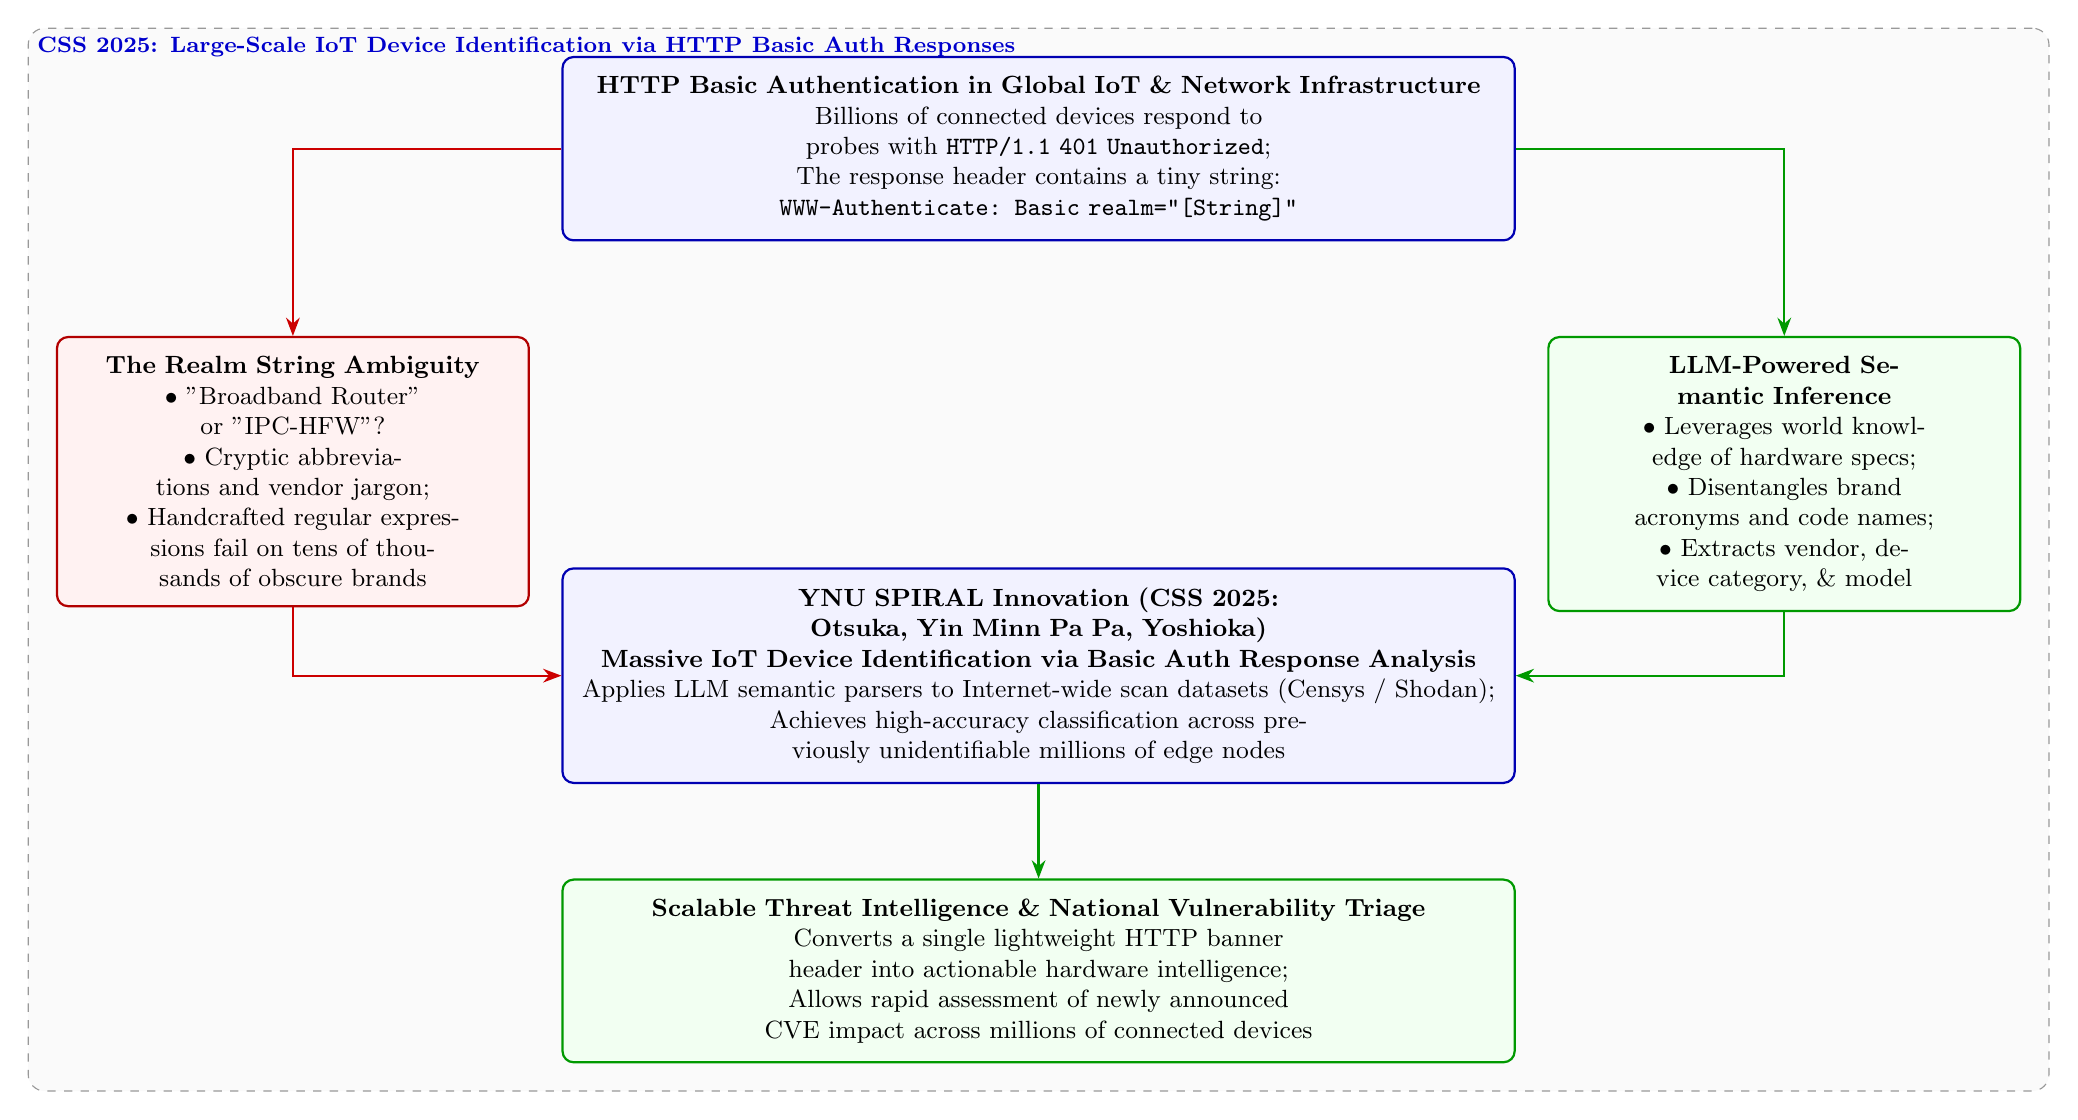
\begin{tikzpicture}[
    font=\small,
    >=Stealth,
    node distance=1.2cm,
    block/.style={rectangle, draw=blue!70!black, fill=blue!5, rounded corners=4pt, thick, align=center, inner sep=7pt},
    alertblock/.style={rectangle, draw=red!70!black, fill=red!5, rounded corners=4pt, thick, align=center, inner sep=7pt},
    greenblock/.style={rectangle, draw=green!60!black, fill=green!5, rounded corners=4pt, thick, align=center, inner sep=7pt},
    amberblock/.style={rectangle, draw=orange!80!black, fill=orange!5, rounded corners=4pt, thick, align=center, inner sep=7pt},
    groupbox/.style={draw=black!40, dashed, rounded corners=6pt, fill=black!2, inner sep=10pt}
]

    % Top: Ubiquitous HTTP 401 Basic Auth
    \node[block, text width=11.6cm] (auth) {\textbf{HTTP Basic Authentication in Global IoT \& Network Infrastructure}\\Billions of connected devices respond to probes with \texttt{HTTP/1.1 401 Unauthorized};\\The response header contains a tiny string: \texttt{WWW-Authenticate: Basic realm="[String]"}};

    % Left: Manual Regex Bottleneck
    \node[alertblock, below left=1.2cm and 0.4cm of auth, text width=5.5cm] (manual) {\textbf{The Realm String Ambiguity}\\$\bullet$ "Broadband Router" or "IPC-HFW"?\\$\bullet$ Cryptic abbreviations and vendor jargon;\\$\bullet$ Handcrafted regular expressions fail on tens of thousands of obscure brands};

    % Right: LLM Contextual Inference
    \node[greenblock, below right=1.2cm and 0.4cm of auth, text width=5.5cm] (llm) {\textbf{LLM-Powered Semantic Inference}\\$\bullet$ Leverages world knowledge of hardware specs;\\$\bullet$ Disentangles brand acronyms and code names;\\$\bullet$ Extracts vendor, device category, \& model};

    \draw[->, thick, red!80!black] (auth) -| (manual);
    \draw[->, thick, green!60!black] (auth) -| (llm);

    % Middle: YNU & Mitsubishi Electric Research (CSS 2025)
    \node[block, below=1.2cm of $(manual)!0.5!(llm)$, text width=11.6cm] (breakthrough) {\textbf{YNU SPIRAL Innovation (CSS 2025: Otsuka, Yin Minn Pa Pa, Yoshioka)}\\\textbf{Massive IoT Device Identification via Basic Auth Response Analysis}\\Applies LLM semantic parsers to Internet-wide scan datasets (Censys / Shodan);\\Achieves high-accuracy classification across previously unidentifiable millions of edge nodes};

    \draw[->, thick, red!80!black] (manual) |- (breakthrough);
    \draw[->, thick, green!60!black] (llm) |- (breakthrough);

    % Bottom: Impact
    \node[greenblock, below=1.2cm of breakthrough, text width=11.6cm] (impact) {\textbf{Scalable Threat Intelligence \& National Vulnerability Triage}\\Converts a single lightweight HTTP banner header into actionable hardware intelligence;\\Allows rapid assessment of newly announced CVE impact across millions of connected devices};

    \draw[->, thick, green!60!black] (breakthrough) -- (impact);

    \begin{scope}[on background layer]
        \node[groupbox, fit=(auth) (manual) (llm) (breakthrough) (impact), label={[anchor=north west, font=\footnotesize\bfseries, blue!80!black]north west:CSS 2025: Large-Scale IoT Device Identification via HTTP Basic Auth Responses}] {};
    \end{scope}

\end{tikzpicture}
\end{document}
